\subsection*{Numerically Controlled Oscillator}
Control when the accumulator flows over. Needs a very fast counter. Overflow amount gets carried over to next cycle.

\begin{figure}[H]
\centering
\tikzstyle{dot} = [draw,shape=circle,fill=black, scale =.3]
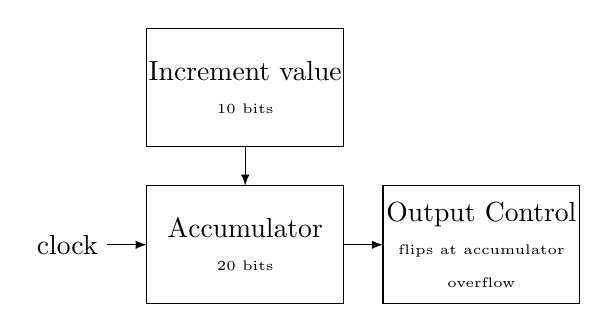
\begin{tikzpicture}


\draw  (0,3) rectangle (2.5,1.5) node[pos=.5, align=center]{Increment value\\\tiny{10 bits}};
\draw  (0,1) rectangle (2.5,-0.5) node[pos=.5, align=center]{Accumulator\\\tiny{20 bits}};
\draw  (3,1) rectangle (5.5,-0.5) node[pos=.5, align=center]{Output Control\\\tiny{flips at accumulator}\\\tiny{overflow}};

\draw [>=latex, ->](2.5,0.25) -- (3,0.25);
\draw [>=latex, ->](-0.5,0.25) -- (0,0.25);
\draw [>=latex, ->](1.25,1.5) -- (1.25,1);
\node [anchor=east] at (-0.5,0.25) {clock};
\end{tikzpicture}
\caption{NCO}
\label{tkz:NCO}
\end{figure}